\chapter{Implementation}
\label{implementation}

This chapter describes the hardware the implementation uses (section \ref{implementation/hardware})
and the developed firmware (section \ref{implementation/software}). The source code for the firmware
can be found at \url{https://github.com/Laegluin/embedded_debug_interface_for_robots/tree/thesis-ref}.
The version referenced by this thesis is tagged as \lstinline{thesis-ref}. The description of the
firmware is intended to give a high level overview and discusses tradeoffs as well as points of
interest.

Since the implementation targets the \textit{Wolfgang} robot platform, it must be compatible with
its \textit{RS-485} bus running at a speed of \SI{2}{\mega{Bd}}.

\section{Hardware}
\label{implementation/hardware}

The following hardware is used:

\begin{itemize}
    \item STM32F7508-DK development board\footnote{\url{https://www.st.com/resource/en/user_manual/dm00537062-discovery-kit-for-stm32f7-series-with-stm32f750n8-mcu-stmicroelectronics.pdf}}
    \item MAX485 RS-485/RS-422 transceiver\footnote{\url{https://datasheets.maximintegrated.com/en/ds/MAX1487-MAX491.pdf}}
    \item FT232R USB to UART converter (for testing)\footnote{\url{https://www.ftdichip.com/Support/Documents/DataSheets/ICs/DS_FT232R.pdf}}
\end{itemize}

The MAX485 transceiver is used to connect the \textit{RS-485} bus to the STM32F7508-DK board. It
outputs a \SI{5}{\volt} signal that can be interpreted by one of the board's UARTs. STM32F7508-DK
is built around a STM32F750N8H6 Arm Cortex-M7 based microcontroller. The controller's \textit{UART6}
is used, as it is easily accessible through the board's Arduino Uno compatible connectors at the
back. All UARTs have a theoretical maximum speed of \SI{27}{\mega{Bd}}~\cite{mcu-ref-manual} (depending
on the clock configuration), making the MAX485's maximum speed of \SI{2.5}{\mega{Bd}} the maximum speed
of this setup~\cite{max-485-manual}\cite{board-user-manual}.

The STM32F7508-DK board has a built in \SI{4.3}{"} 480x272 LCD-TFT capacitive touchscreen. It is
used to display and interact with the UI. Because it is built in, no further assembly is required~\
\cite{board-user-manual}.

The STM32F750N8H6 microcontroller is based on an Arm Cortex-M7 CPU. It supports clock speeds of up to
\SI{216}{\mega\hertz} and has both data and instruction caches. It is equipped with a single-precision
FPU (floating point unit) and a DMA controller~\cite{mcu-datasheet}. While this is quite a lot of
processing power for a microcontroller, it is needed to drive an interactive UI while at the same time
processing incoming data quickly enough. The DMA controller allows transferring data from the UART to
memory at high data rates without using up CPU time.

\begin{figure}[h]
    \centering
    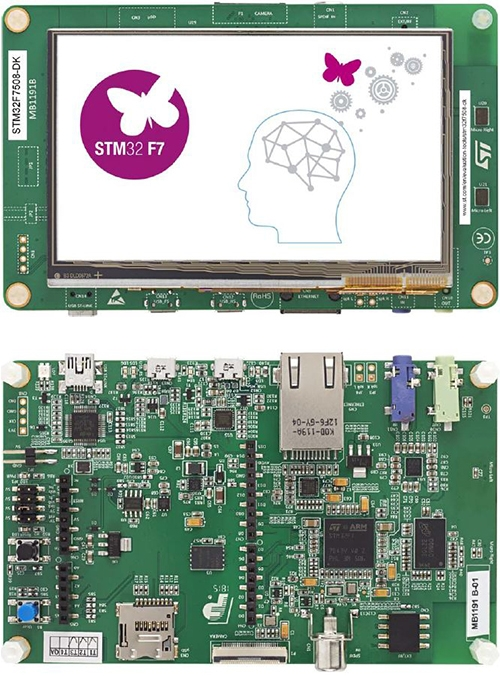
\includegraphics[scale=0.4]{img/board.jpg}
    \caption[The STM32F7508-DK development board]{
        The STM32F7508-DK development board\footnotemark
    }
\end{figure}
\footnotetext{
    Source: \url{https://www.st.com/bin/ecommerce/api/image.PF267270.en.feature-description-include-personalized-no-cpn-large.jpg}
    (Accessed: 2020-03-30)
}

The controller itself comes with only \SI{64}{KiB} of embedded flash memory. However, it also has a
Quad-SPI memory interface that can be used with external flash memory~\cite{mcu-datasheet}. The
STM32F7508-DK board has \SI{16}{MiB} of pre-installed flash memory~\cite{board-user-manual}.

Similarly, \SI{320}{KiB} of RAM are embedded in controller~\cite{mcu-datasheet}. This is more than
enough for most applications but not enough for the video RAM (VRAM) used by the display. When using
double buffering and 8 bits per pixel, at least $480 \cdot 272 \cdot 3 \cdot 2 = 765\,\si{KiB}$ are
needed for VRAM alone. VRAM can be located in external RAM which can be controlled by the microcontroller's
FMC (flexible memory controller). The board has \SI{8}{MiB} of pre-installed external RAM~\
\cite{mcu-datasheet}\cite{board-user-manual}.

The STM32F7508-DK board is equipped with an ST-LINK/V2-1 in-circuit debugger. It can be used for
debugging and for programming the internal flash memory~\cite{board-user-manual}. External flash
cannot be programmed using the ST-LINK; instead a standalone bootloader must be used (see subsection
\ref{implementation/software/bootloader}).

The FT232R USB to UART converter is only used for testing and benchmarking. It can easily be connected
to \textit{UART6} instead of the MAX485. Data can then be sent to the USB serial port emulated by
the FT232R from the computer connected to it~\cite{ftdi-232r-datasheet}. This makes testing extremely
easy since the device can be treated as a serial terminal.

\section{Software}
\label{implementation/software}

This section describes the firmware for the STM32F7508-DK board. The bootloader is written in C
(C99), the actual firmware itself is written in C++ (C++14). All code is compiled with the
\textit{GNU arm-none-eabi} toolchain. \textit{Newlib} is used as the C standard library implementation.

\subsection{Bootloader}
\label{implementation/software/bootloader}

When the microcontroller is reset, it loads the \textit{vector table} from address \mbox{\lstinline{0x00000000}.}
The \textit{vector table} contains the addresses of all possible interrupt handlers. In addition, the
first item is the initial value of the stackpointer and the second is the address of the entry point.
After loading the \textit{vector table}, the stackpointer is set to the configured value and the
processor jumps to the entry point~\cite{mcu-ref-manual}. By default, addresses in the range
\lstinline{[0x00000000, 0x08000000)} are mapped to \lstinline{0x08000000}, which in turn is mapped
to internal flash memory~\cite{mcu-ref-manual}.

This poses a problem for applications that do not fit into internal flash memory: there is no way to
boot from the much larger Quad-SPI flash memory or to program it. An additional bootloader has to be
used instead. A bootloader is a minimal application that initializes a peripheral device for I/O,
accepts commands as well as data from said device and allows programming and booting from otherwise
unsupported memory.

In this case, the bootloader must allow programming and booting from Quad-SPI flash memory. It uses
one of the STM32F7508-DK board's micro-USB ports for I/O~\cite{board-user-manual}. USB is a well
suited interface because data integrity checks are built in~\cite{usb-2-spec}. STMicroelectronics
provides a USB 2.0 compliant library for applicable microcontrollers that the bootloader uses for
USB support~\cite{stm32-usb-lib}.

When the bootloader starts, it initializes the USB controller and the Quad-SPI memory interface. It
also blinks the board's LED at regular intervals to indicate that it is running. It then listens on
the USB interface as a communication class device.

\begin{figure}[ht]
    \centering

    \begin{subfigure}[t]{0.5\textwidth}
        \centering
        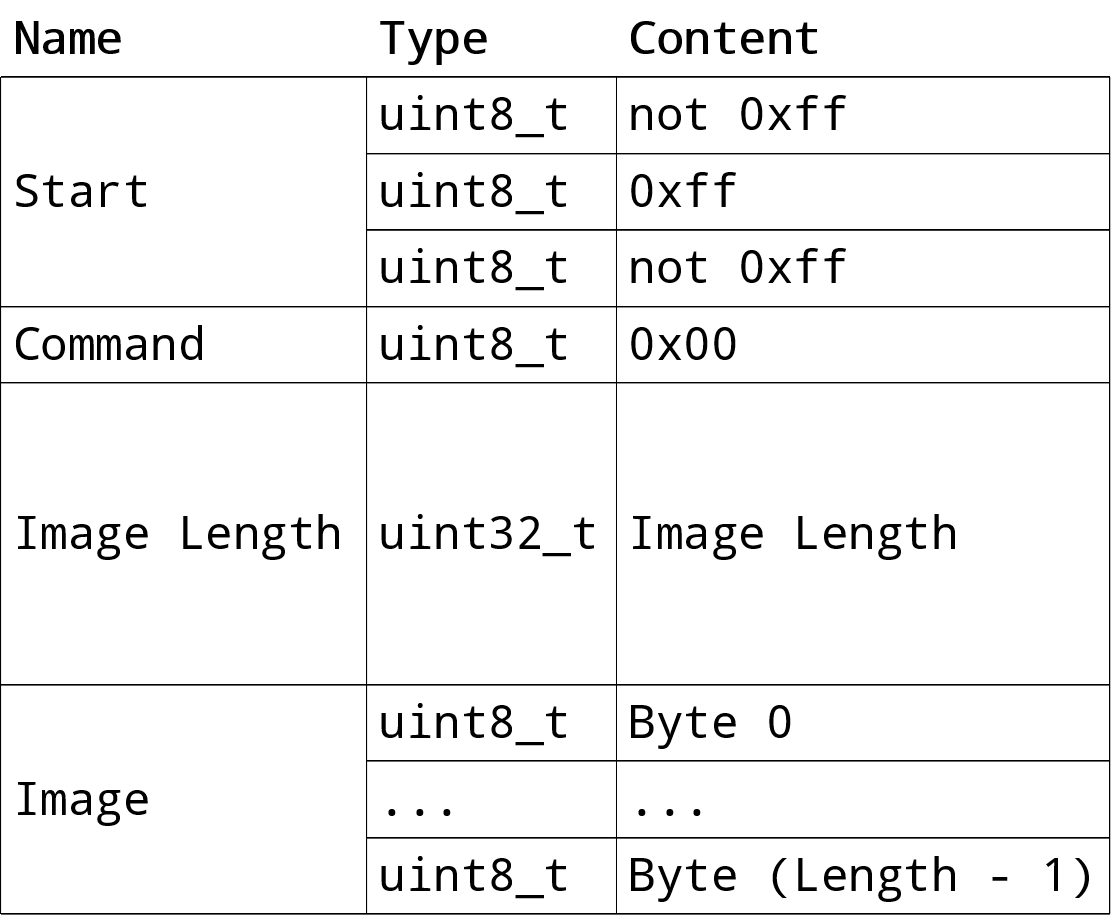
\includegraphics[scale=0.18]{img/bootloader_flash_packet.png}
        \caption{\textit{flash} packet layout}
    \end{subfigure}%
    \begin{subfigure}[t]{0.5\textwidth}
        \centering
        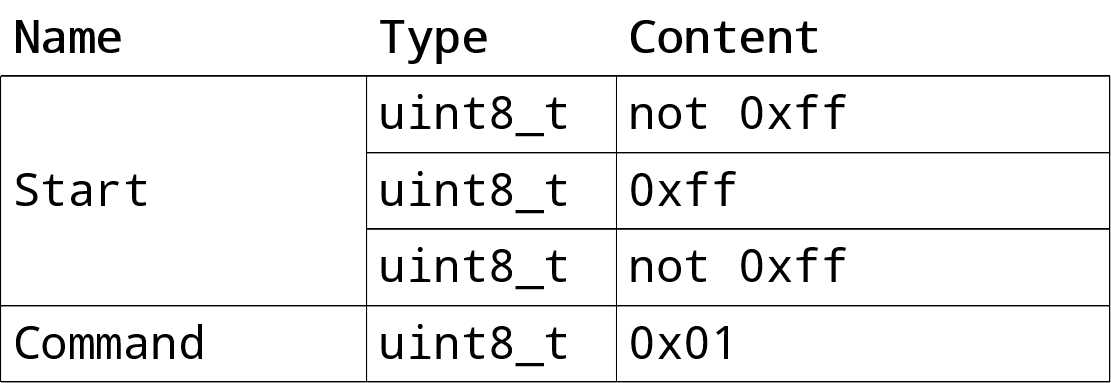
\includegraphics[scale=0.18]{img/bootloader_start_packet.png}
        \caption{\textit{start} packet layout}
    \end{subfigure}

    \caption{Bootloader packet layout}
    \label{implementation/software/bootloader/packet-layout}
\end{figure}

The bytes received are interpreted according to a custom, packet based protocol. The packet layout
can be seen in figure \ref{implementation/software/bootloader/packet-layout}. Packets start with a
start sequence that makes it possible to identify the beginning of a packet even if it is preceded
by unrelated bytes. To prevent unwanted start sequences in the packet itself, all bytes following
the start sequence must be escaped by adding \textit{byte stuffing}: whenever a byte that is not
\lstinline{0xff} is followed by a \lstinline{0xff} byte, another \lstinline{0xff} byte must be added.
For example, the bytes \lstinline{0x00 0xff 0xff} must be sent as \lstinline{0x00 0xff 0xff 0xff}.
The bootloader simply removes the added bytes before processing the rest. Values of more than one
byte are encoded as \textit{little-endian} and lengths are always given as the length before any
\textit{byte stuffing} was applied.

A \textit{flash} packet instructs the bootloader to erase and then program the Quad-SPI flash memory
with all the bytes in the \textit{Image} field, beginning at the start address of the Quad-SPI flash
memory.

\begin{figure}[ht]
    \centering
    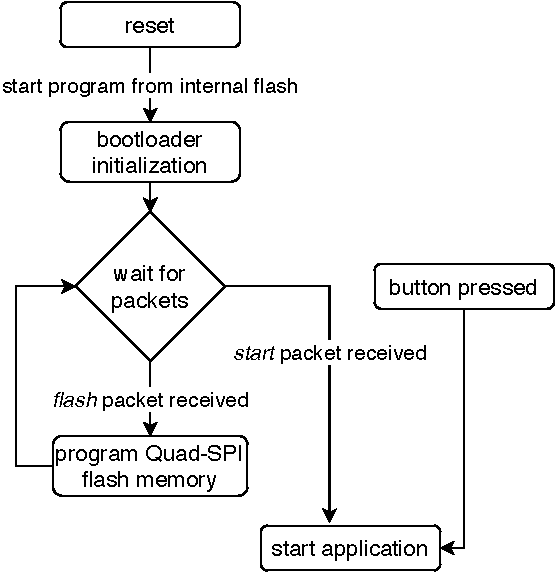
\includegraphics[scale=1.0]{img/bootloader_flowchart.pdf}
    \caption[Bootloader program flow]{
        After reset, the microcontroller starts the program in internal flash memory (the bootloader).
        It then waits for packets to arrive over USB. If a \textit{start} packet has been received or
        the button was pressed, it starts the application in Quad-SPI flash memory.
    }
\end{figure}

The \textit{start} packet instructs the bootloader to start an application previously flashed. It
disables all (pending) interrupts, exits interrupt handler mode if necessary and enables the
memory-mapped mode for the Quad-SPI memory interface. In addition it also enables the board's LED
permanently, indicating that the application is now running. Finally, it starts the application by
loading the stackpointer and jumping to the entry point in the same way the microcontroller does
when it boots from internal flash memory. The bootloader assumes that the application's \textit{vector table}
starts at the beginning of the Quad-SPI flash memory space (\lstinline{0x90000000}~\cite{mcu-ref-manual}).
The application can also be started by pressing the board's programmable button (next to the reset
button). The procedure is identical to the one described above.

The bootloader only has to be flashed to internal flash memory once. Afterwards, it can be used to
program the Quad-SPI flash memory and start an application from it using the board's micro-USB port.
In this case, the application is the actual firmware that controls the UI and processes packets
sent over the \textit{Wolfgang} robot platform's \textit{RS-485} bus.

\subsection{Used Libraries}
\label{implementation/software/used-libraries}

The following software libraries were used to aid development of the firmware:

\begin{itemize}
    \item STM32F7 HAL and Low-layer drivers\footnote{\url{https://www.st.com/resource/en/user_manual/dm00189702-description-of-stm32f7-hal-and-lowlayer-drivers-stmicroelectronics.pdf}}
          (part of STM32CubeF7 1.15.0)
    \item STM32F7508-Discovery board support package\footnote{\url{https://github.com/STMicroelectronics/STM32CubeF7/tree/master/Drivers/BSP/STM32F7508-Discovery}}
          (part of STM32CubeF7 1.15.0)
    \item STemWin version 5.44 (part of STM32CubeF7 1.15.0)
    \item FreeRTOS\footnote{\url{https://www.freertos.org/}} version 10.0.1 (part of STM32CubeF7 1.15.0)
    \item Catch2\footnote{\url{https://github.com/catchorg/Catch2}} version 2.10.2
\end{itemize}

The STM32F7 HAL and Low-layer drivers are various independent drivers for peripherals found on
hardware produced by STMicroelectronics. Despite the name (HAL - hardware abstraction layer) they
still require the user to write hardware specific code. They do offer simplified interfaces that do
not require manipulation of memory-mapped peripheral device registers. For more complicated peripherals
like the LCD controller this can be helpful~\cite{stm32-hal-docs}.

Similarly, the STM32F7508-Discovery board support package offers drivers based on the HAL and
Low-layer drivers that are customized for the STM32F7508-DK board. They encapsulate all of the
hardware and have easier to use interfaces than their HAL counterparts~\cite{stm32-cube-getting-started}.

STemWin is GUI library based on emWin by SEGGER Microcontroller GmbH \& Co. KG. It is effectively
a precompiled version of emWin with driver support for STMicroelectronics' hardware. While emWin is
commercially licensed, STemWin is licensed as free of charge for use with STMicroelectronics' products~\
\cite{stm32-cube-getting-started}\cite{stemwin-release-notes}\cite{emwin-manual}. Since it is otherwise
indistinguishable from emWin, it will be referred to as emWin in the following. emWin was chosen instead
of TouchGFX (also part of STM32CubeF7) because it does not require code generation and has extensive
documentation.

FreeRTOS is a popular embedded operating system. It is permissively licensed and widely used by major
companies. It is specifically designed to run with minimal overhead (both code size and execution
speed)~\cite{freertos-about}. STMicroelectronics provides a distribution of FreeRTOS that is already
configured for their microcontrollers as part of STM32CubeF7~\cite{stm32-cube-getting-started}.

Catch2 is a unit testing library for C++11 and above. Tests are written as simple functions with
assertions and do not require complex setup. It is a header-only library, meaning that no additional
build system configuration is necessary~\cite{catch2-why}.

\subsection{Testing}
\label{implementation/software/testing}

Automatic testing of the hardware specific code and the UI is difficult. Tests concerning the bus
were done using the FT232R USB to UART converter to send test data as well as traces of real bus
traffic directly to microcontroller's UART. UI tests were also performed manually, usually as part
of the aforementioned tests.

Most of the core logic deals with data received over the bus. The actual origin of the data is not
relevant for testing. This code is carefully structured to avoid any dependencies on hardware 
specific code. It is tested using Catch2 unit tests running on the host platform (Linux on AMD64).
While this is not a perfect solution as there are still differences between the platforms like pointer
sizes, alignment requirements or hardware protection mechanisms provided by the operating system,
it creates high confidence in the correctness of the code nevertheless.

In addition, manual tests on a real robot were also performed whenever possible. Due to the high
setup time these tests were intended as a final quality measure and not as a general tool for finding
bugs.

\subsection{Overview}
\label{implementation/software/overview}

On startup the firmware first configures the required peripheral devices. This includes the UART
(specifically \textit{UART6}), the LCD controller and the external RAM used as frame buffer for emWin.
Care must be taken when using the external RAM in combination with another device (the LCD controller
in this case) as external RAM is cached by the CPU. Since the LCD controller does not know about
any CPU caches, writes to the frame buffers will not be visible to it until the writes are flushed
to memory, causing visible artifacts on the screen~\cite{mcu-ref-manual}.

This can be prevented by using the microcontroller's MPU (memory protection unit). The MPU allows
disabling write caching for certain memory regions~\cite{mcu-ref-manual}. Reads can still be cached,
since only the CPU writes to the frame buffer. Additionally, the MPU is also used to disable access
to a \SI{4}{KiB} region starting at \lstinline{0x00000000}. This helps catch dereferences of 
\textit{null}-pointers---a common programming error---early. Otherwise, \textit{null}-pointer
dereferences would be perfectly valid, since the address \lstinline{0x00000000} is mapped to the
start of the internal flash memory (see subsection \ref{implementation/software/bootloader}).

Finally, the FreeRTOS scheduler has to be started. It takes over the execution and starts scheduling
tasks (FreeRTOS uses this term instead of thread). The \textit{SysTick}, \textit{SVCall} and
\textit{PendSV} interrupts must use the handlers provided by FreeRTOS in order for FreeRTOS to
function correctly. The \textit{SysTick} interrupt must also run at the lowest possible interrupt
priority~\cite{freertos-arm-cortex-m}. This conflicts with STMicroelectronics' HAL library, which
expects to be called from the \textit{SysTick} interrupt running at the highest priority~\cite{stm32-hal-docs}.
As a workaround, the HAL library is called from a separate timer interrupt that is running at the
highest priority and identical frequency to the \textit{SysTick} interrupt.

Since tasks scheduled by FreeRTOS run concurrently, it is necessary to secure any shared state against
concurrent accesses. This also applies to \textit{Newlib}, the C standard library implementation
that is used. Its \lstinline{malloc} implementation is used for all heap allocations in the standard
library, including C++ containers like \mbox{\lstinline{std::vector},} but is not safe to use concurrently~\
\cite{newlib-malloc-lock}. There are ways to secure it by providing a global lock; however, FreeRTOS
already includes an optimized concurrency safe memory allocator~\cite{freertos-allocators}. The linker's
\lstinline{--wrap} option~\cite{arm-none-eabi-ld-manpage} is used to replace the malloc function with
a custom implementation that simply calls the FreeRTOS allocator. This way all code automatically
uses the correct allocator.

There are two tasks that have to run concurrently: one is processing incoming data and the other is
updating the UI. Both of these tasks share two data structures that are each protected by a mutex.
The \lstinline{Log} object stores recent errors and profiling information whereas the
\lstinline{ControlTableMap} stores all currently known information about devices connected to the
\textit{RS-485} bus (for more detail see \ref{implementation/software/packet-processing-task}).

The packet processing task runs at higher priority than the UI task. This means it will run until
it deliberately yields control to lower priority tasks for a short amount of time. This way the UI
task only gets a limited amount of processing time, leaving the rest for packet processing. If the
UI task is currently holding the lock on a mutex and the packet processing task is trying to lock the
same mutex, the FreeRTOS scheduler temporarily assigns the priority of the packet processing task
to the UI task (priority inheritance). The UI task can now run until it releases the lock, at which
point it reverts to its previous priority and is preempted by the packet processing task~\
\cite{freertos-create-mutex-docs}. Again, the UI task only runs as long as it has to, freeing the
rest of the time for packet processing.

The following two subsections describe the design of the two tasks in more detail. Subsection
\ref{implementation/software/ui-task} describes the UI task, subsection
\ref{implementation/software/packet-processing-task} the packet processing task.

\subsection{UI Task}
\label{implementation/software/ui-task}

The UI task is responsible for updating and drawing the UI as well as processing touch input. The
task simply consists of an infinite loop calling the emWin function \mbox{\lstinline{GUI_Exec},}
which handles user input and timers. A separate hardware timer interrupt polls the touch controller
at \SI{30}{\hertz} and stores updates to its state in emWin's input queue.

\begin{lstlisting}[language=C++, caption={Main loop of the UI task}]
while (true) {
    GUI_Exec();
}
\end{lstlisting}

In emWin, every part of the user interface is a window: windows themselves, buttons, scrollbars,
lists, etc. Every window is identified by a \textit{handle}. A \textit{handle} is an integer that
emWin associates with a window. All functions operating on a window take its handle as an argument.
Some of these functions only apply to some types of windows, like for example functions for
manipulating buttons~\cite{emwin-manual}.

Every window also has a \textit{callback} function associated with it. This function is called whenever
the window receives a messages. Messages can be user input, elapsed timers, notifications from other
windows or even a request to draw itself. \textit{Callbacks} can be overridden by supplying a new
function to use instead. Often, this function only handles some messages and delegates the remaining
messages to the original \textit{callback} function. Most importantly, \textit{callbacks} are a way
to react to user input on a specific window~\cite{emwin-manual}.

The goal of the UI is to make it easy to identify the status of devices at a glance. It is split
into three separate views, each displaying information at a different level of detail: the device
overview, the model overview and the device details view. A fourth view displays profiling information
and log messages. Every view is a distinct window that covers the entire screen. Color coding is used
to differentiate between connected and disconnected devices. Every list item or button representing
a connected device is colored green, those representing disconnected devices are colored red. The
following four paragraphs give a brief overview of each view.

\clearpage
\paragraph{Device overview}

Displays the total number of devices and the number of devices for each model. It is the view shown
when the application is started and is meant to give a brief summary for all devices. Each summary
for a certain model can be clicked to open the model overview of that model. It also features buttons
to reach the device details view and the log view. While this view does not provide much detail,
disconnected devices are immediately visible. The view is updated every \SI{500}{\milli\second}.

\begin{figure}[H]
    \centering
    \setlength{\fboxsep}{0mm}
    \fbox{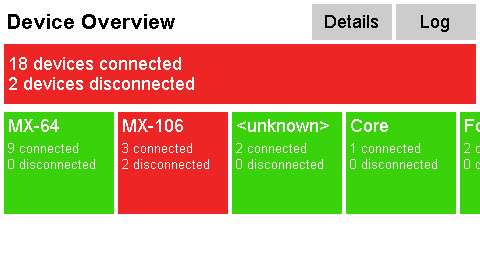
\includegraphics[scale=0.75]{img/device_overview.png}}
    \caption[Screenshot of the device overview]{
        Screenshot of the device overview. The top bar is red because at least one device (two in
        this case) is disconnected. The squares below the bar show the status of the devices of a
        specific model. They also turn red if at least one device is disconnected. The list containing
        them is horizontally scrollable. Each square can be clicked and will open the model overview
        for the corresponding model.
    }
\end{figure}

\clearpage
\paragraph{Model overview}

Displays the status and ID of each device of a certain model. Each device in the list can be clicked
to open the device details view and select that device. This view does not provide as much detail as
the device details view but it only shows devices of one particular model, making it easy to find
the exact device that is disconnected. The view is updated every \SI{500}{\milli\second}.

\begin{figure}[H]
    \centering
    \setlength{\fboxsep}{0mm}
    \fbox{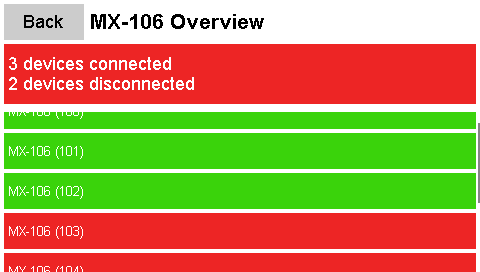
\includegraphics[scale=0.75]{img/model_overview.png}}
    \caption[Screenshot of the model overview]{
        Screenshot of the model overview. The top bar is red because at least one device for the
        selected model (MX-106) is disconnected. Below the bar is a scrollable list with an item for
        each device of the selected model. The device's ID is shown in parentheses and the item is
        colored red when it is disconnected. Clicking an item will navigate to the device details view
        and select the clicked device.
    }
\end{figure}

\clearpage
\paragraph{Device details view}

Displays all known values of single device's \textit{control table}. Different devices can be selected
by using the list on the left hand side. This view provides the maximum amount of detail per device
but makes it harder to determine the status of all connected devices at once. The view is updated every
\SI{500}{\milli\second}.

\begin{figure}[H]
    \centering
    \setlength{\fboxsep}{0mm}
    \fbox{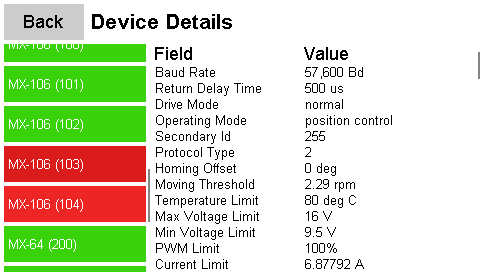
\includegraphics[scale=0.75]{img/device_details_view.png}}
    \caption[Screenshot of the device details view]{
        Screenshot of the device details view. The list on the left hand side contains an item for
        each connected device that is colored green when the device is connected and red otherwise.
        Clicking an item will select that device and show all values of its \textit{control table}
        in the table on the right hand side.
    }
\end{figure}

\clearpage
\paragraph{Log view}

Displays profiling information such as free memory and maximum and average processing times, as well
as the last 50 errors that occurred during packet processing. This view is mostly intended for debugging.
It has to be refreshed manually since a lot of errors may occur in short bursts, making it impossible
to actually read an individual error message.

\begin{figure}[H]
    \centering
    \setlength{\fboxsep}{0mm}
    \fbox{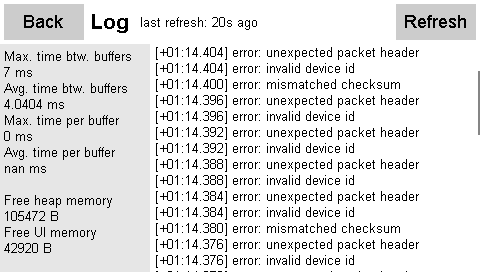
\includegraphics[scale=0.75]{img/log_view.png}}
    \caption[Screenshot of the log view]{
        Screenshot of the log view. The left hand side contains profiling information like processing
        times and free memory, the right hand side shows the 50 most recent error messages. The
        timestamps in the error log are relative to the start of the application. The view is only
        refreshed when the \textit{Refresh} button is clicked.
    }
\end{figure}

All of the views have to regularly access data shared with the packet processing task. While they
are holding the lock for this data, the packet processing task may be blocked on this lock. This
makes it extremely important to minimize the time spent holding any locks. All of the views do this
by copying the needed data before processing it. Thus, they only ever hold a lock to make copies,
which is relatively quick compared to updating the entire UI at the same time. This does decrease
the theoretical performance of the UI; however, the UI only needs to be fast enough to not appear
slow to the user. In comparison, the packet processing task has strict deadlines. If it is blocked
for too long, it will miss incoming data.

\subsection{Packet Processing Task}
\label{implementation/software/packet-processing-task}

The packet processing task is responsible for processing the data the UART connected to the \textit{RS-485}
bus receives. Since the bus has a data rate of \SI{2}{\mega{Bd}}, performance is crucial. Data must be
processed faster than it arrives in order to not lose any of it. At the same time, there needs to be
enough processing time left to also update to UI.

The code is designed to work with more than one bus at the same time. Each bus is associated with
a \lstinline{Connection} object. It holds the state of the packet parser, some profiling information
and a pointer to a buffer that stores received data. At the moment, only a single bus connected to
\textit{UART6} is supported.

\begin{lstlisting}[language=C++, caption={Main loop of the packet processing task}]
while (true) {
    for (auto& connection : connections) {
        if (connection.last_processing_start == 0) {
            connection.last_processing_start = HAL_GetTick();
        }

        process_buffer(log, connection, control_table_map);
    }

    vTaskDelay(4 / portTICK_PERIOD_MS);
}
\end{lstlisting}

The buffer is automatically filled by the DMA controller. It transfers the bytes from the UARTs
receive register and raises interrupts when half or the entire buffer has been filled. Once it has
been filled, the DMA controller starts at the beginning of the buffer again. The interrupt handler
sets a flag that determines which part of the buffer is now ready. As long as the data is processed
faster than it is received, no data will be lost. Even when the data is not processed quickly enough,
there will be no serious malfunctions. Some data may be corrupted but this will usually be detected
by the CRC checksums that are part of the ROBOTIS Dynamixel protocol (see section \ref{basics/dynamixel-protocol}).

The size of the buffer has a significant impact on the maximum time allowed before data is lost. A
larger buffer increases this time but also increases the latency. The latency can largely be ignored
because it is still low (for human time scales) given the possible buffer sizes. Latency would
increase drastically if there were no or only very little traffic on the bus, as data is only ever
processed once one half of the buffer is ready. Other than by memory contraints, the size of the buffer
is limited to \SI{65535}{B} by the size of the DMA controller's NDT register~\cite{mcu-ref-manual}.

The buffer's size is \SI{8192}{B}. This means that even assuming the absolute worst case, the maximum
amount of time for processing one half of the buffer is
$\frac{\SI{4096}{B}}{\SI{2}{\mega{Bd}} \mathbin{/} 8} \approx \SI{16}{\milli\second}$. Realistically,
the maximum amount of time will be higher for multiple reasons:

\begin{itemize}
    \item The baud rate of the bus is not equivalent to the bit rate of the incoming data, since
          this equation ignores overhead like stop bits.
    \item In practice it is impossible to have \SI{100}{\percent} load on the bus.
    \item The equation assumes that processing starts right after an interrupt signals that one half
          of the buffer is ready, and does not actually process a single byte. Normally, data is
          then being processed, which continuously moves the point at which a collision with the DMA
          controller can occur.
\end{itemize}

For these reasons, if the maximum amount of time between processing one half of the buffer never
exceeds \SI{16}{\milli\second}, there will be no data loss or corruption.

\begin{figure}[h]
    \centering
    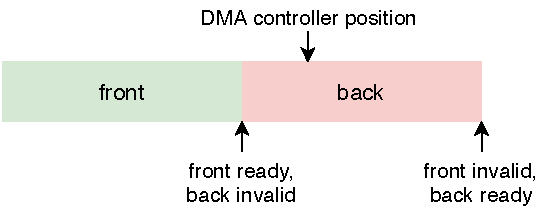
\includegraphics[scale=1.0]{img/dma_buffer.pdf}
    \caption[Layout of the DMA buffer]{
        After more than half of the DMA buffer has been filled, the front of it is ready and can be
        read. At the same time, the back of it is now invalid because the DMA controller is writing
        to it. The situation is reversed when the DMA controller has finished writing to the back
        and starts at the front again.
    }
\end{figure}

Since the buffer is written to by the DMA controller and then read by the CPU, the CPU must not cache
reads. This is accomplished by placing the buffer in the DTCM RAM section of the microcontroller's
memory. DTCM RAM is never cached~\cite{mcu-ref-manual}.

After processing one half of each buffer per bus, control is yielded to the UI task for \SI{4}{\milli\second}.
The UI can only be updated during this time. Increasing this time also increases the responsiveness
of the UI while increasing the time spent between the processing of data.

The \lstinline{process_buffer} function then parses packets until all the data in the ready buffer
has been consumed. Each successfully parsed packet is passed to \lstinline{ControlTableMap::receive},
which processes the contents of the packets. Errors and profiling information are passed to the
\lstinline{Log} object afterwards.

Due to this, the mutexes for the \lstinline{ControlTableMap} and the \lstinline{Log} object are
never locked at the same time. The UI task also never locks more than one of these mutexes at a time.
Holding only one lock at the same time prevents deadlocks.

The lock for the \lstinline{ControlTableMap} object is intentionally is held for almost the whole
duration of the call. Unlike with the UI task where holding the lock for a long time would block
the packet processing task, there is no task to block since the only other task is the UI task which
can only run when the packet processing explicitly yields control. Maximizing the time holding a
mutex removes the overhead of locking it multiple times.

\paragraph{Parser}

The \lstinline{Parser} is responsible for parsing packets from the ready part of a buffer. It
consumes bytes from a \mbox{\lstinline{Cursor}.} A \lstinline{Cursor} is essentially a pointer to
a part of the buffer that also tracks how many bytes have already been read. This enables a simple
API for the \lstinline{Parser} itself. Each call to the \lstinline{parse} method either parses one
packet successfully, encounters an error or parses a packet partially. In all cases, the \lstinline{Cursor}
tracks the current position and indicates when all bytes have been consumed, while the \lstinline{Parser}
holds state that must be retained across parses.

Most importantly, it stores the previous three bytes. When inspecting the next byte there are three
possible scenarios:

\begin{itemize}
    \item the byte and the previous three bytes are the header of a new packet
    \item the byte is stuffing (it can be ignored)
    \item the byte is a regular byte
\end{itemize}

In case the header of a packet is detected while already parsing a packet, an error is returned.
Returning early when encountering an error or only partially parsing a packet is possible because
the \lstinline{Parser} stores the part of the packet currently being parsed and the incremental
CRC checksum.

\begin{lstlisting}[language=C++, caption={Definition of the \lstinline{Packet} struct}]
struct Packet {
    DeviceId device_id;
    Instruction instruction;
    Error error;
    std::vector<uint8_t> data;
};
\end{lstlisting}

The speed of the \lstinline{Parser} is critical to performance. To avoid allocating memory while
parsing, the \lstinline{parse} method takes a pointer to a \lstinline{Packet} struct as argument.
Since packets are processed sequentially, the same \lstinline{Packet} struct can be reused. Packets
themselves can have different lengths but when defining a maximum allowed packet length, the memory
for a \lstinline{Packet} of that length can be preallocated. Defining a maximum packet length also
makes sense in order to avoid running out of memory due to packets with incorrect \textit{Length}
fields.

The \lstinline{Packet} struct represents both instruction and status packets since the only difference
between them is the addition of an \textit{Error} field for status packets (see section
\ref{basics/dynamixel-protocol}). For instruction packets the \lstinline{error} member can be ignored
because it will never contain an error.

\paragraph{ControlTableMap}

The \lstinline{ControlTableMap} object then processes these \lstinline{Packet} structs further.
Status packets are left as is but instruction packets are parsed into \lstinline{InstructionPacket}
structs. An \lstinline{InstructionPacket} is a discriminated union of structs for each instruction.
Because the instruction specific fields are part of the payload of a packet, parsing them is simple.
Unlike the packet parser, the instruction packet parser is just a function. It also reuses previous
\lstinline{InstructionPacket}s, but does allocate memory. Further optimization was not required to
achieve the desired performance.

\begin{lstlisting}[language=C++, caption={Definition of the \lstinline{InstructionPacket} struct}]
struct InstructionPacket {
    // constructors, destructor and member functions omitted

    Instruction instruction;
    union {
        PingArgs ping;
        ReadArgs read;
        WriteArgs write;
        RegWriteArgs reg_write;
        ActionArgs action;
        FactoryResetArgs factory_reset;
        RebootArgs reboot;
        ClearArgs clear;
        SyncReadArgs sync_read;
        SyncWriteArgs sync_write;
        BulkReadArgs bulk_read;
        BulkWriteArgs bulk_write;
    };
};
\end{lstlisting}

For every received instruction packet, the \lstinline{ControlTableMap} records the devices that are
expected to respond. When a new instruction packet is received, a counter for each device from which
a status packet was not received is incremented. These counters are reset when a status packet from
the corresponding device has been received. Devices that have not responded to more than four instruction
packets are considered disconnected.

\textit{Ping} instructions are handled differently: the status packet responding to a \textit{Ping}
instruction contains the model number of the device. The model number is used to register a new device.
Each device is mapped to a \lstinline{ControlTable} object that stores the current state of the device's
\textit{control table}. If the device is not registered, has a different or an unknown model number,
a new \lstinline{ControlTable} matching the model number is allocated. A device's model can be unknown
if status packets from that device have been received without previously receiving the response to a
\textit{Ping} instruction.

Whenever data is written to or read from a device, the written or read data is also updated for the
\lstinline{ControlTable} object belonging to that device. This is the data that is displayed by the
UI. Only the following instructions are handled properly:

\begin{itemize}
    \item \textit{Ping}
    \item \textit{Read}
    \item \textit{Write}
    \item \textit{Sync Read}
    \item \textit{Sync Write}
    \item \textit{Bulk Read}
    \item \textit{Bulk Write}
\end{itemize}

The remaining instructions are mostly ignored but still used for detecting disconnected devices.
Adding support for them would be a significant effort especially considering that these instructions
do not appear in most traffic. The current implementation also assumes that writes do not require a
status packet response, as this is how the \textit{Wolfgang} robot platform is configured.

The \lstinline{ControlTable} objects are identified by the ID of the device they belong to. Initially,
a \lstinline{std::unordered_map} was used but the performance proved to be insufficient. Instead, the
objects are stored in a custom data structure. It takes advantage of the fact that device IDs are
only one byte and that \lstinline{ControlTable} objects must be accessed through a pointer (four bytes
on a Cortex M7 processor~\cite{mcu-ref-manual}). The objects are simply stored in an array that is
indexed by the device ID. An additional boolean flag indicates presence or absence of the object. The
entire array only requires $256 \cdot (4 + 1 + 3) = \SI{2048}{B}$ of memory (this includes three bytes
of padding).
This solution trades memory and iteration speed for fast access times. Since objects must be accessed
for almost every received packet, this provides a serious speedup compared to \lstinline{std::unordered_map}.

\paragraph{ControlTable}

The \textit{control table} of each device is represented by a \lstinline{ControlTable} object. For
each device model there is a different sub class of \lstinline{ControlTable}. Most received packets
update the \lstinline{ControlTable} object of at least one device, performance is thus an important
design consideration. Adding or changing the \lstinline{ControlTable} of a device has to be easy.

The interface definition of the \lstinline{ControlTable} base class can be seen in listing
\ref{implementation/software/packet-processing-task/control-table-def}. \lstinline{is_unknown_model}
determines if the model number is known and \lstinline{model_number} returns its value if present.
\lstinline{set_firmware_version} is called when the firmware version is reported by the response
to a \textit{Ping} instruction. \lstinline{device_name} simply returns a human readable name of the
model represented by the \lstinline{ControlTable}. It is used for display purposes only.

\begin{lstlisting}[
    language=C++,
    caption={Definition of the \lstinline{ControlTable} class},
    label=implementation/software/packet-processing-task/control-table-def,
]
class ControlTable {
  public:
    virtual ~ControlTable() = default;

    virtual std::unique_ptr<ControlTable> clone() const = 0;

    virtual bool is_unknown_model() const;

    virtual uint16_t model_number() const = 0;

    virtual void set_firmware_version(uint8_t version) = 0;

    virtual const char* device_name() const = 0;

    virtual ControlTableMemory& memory() = 0;

    virtual const ControlTableMemory& memory() const = 0;

    virtual const std::vector<ControlTableField>& fields() const = 0;

    bool write(uint16_t start_addr, const uint8_t* buf, uint16_t len);

    std::vector<std::pair<const char*, std::string>> fmt_fields() const;
};
\end{lstlisting}

The core functionality of \lstinline{ControlTable} class uses the \lstinline{memory} and
\lstinline{fields} methods. The \lstinline{ControlTableMemory} object returned by a call to
\lstinline{memory} is responsible for storing the actual data. It is made up of multiple
\lstinline{Segment}s that each describe a region of memory:

\begin{itemize}
    \item data segments are some memory starting at a certain address
    \item indirect address segments allow redirecting addresses (required to support ROBOTIS
          \textit{MX-64} and \textit{MX-106} servos)
    \item unknown segments allow no reads and ignore writes (these are used when the model number
          is not known)
\end{itemize}

The descriptions are used by the \lstinline{ControlTableMemory} object to map data contained in
packets to a single, flat byte array. Calls to the \lstinline{write} method of a \lstinline{ControlTable}
object are forwarded to the \lstinline{ControlTableMemory}. By using an accessor, only one virtual
call has to be performed, even when writing more than one byte.

The \lstinline{fields} method returns a description of all fields in a device's \textit{control table}.
Each \lstinline{ControlTableField} stores the address, type, name, and default value of a single
field. It also contains a function for formatting the value of the field as a human readable string.

\begin{lstlisting}[language=C++, caption={Definition of the control table fields of a Rhoban DXL Board}]
const std::vector<ControlTableField> CoreBoardControlTable::FIELDS{
  ControlTableField::new_uint16(0, "Model Number", CoreBoardControlTable::MODEL_NUMBER, fmt_number),
  ControlTableField::new_uint8(2, "Firmware Version", 0, fmt_number),

  ControlTableField::new_uint16(10, "LED", 0, fmt_bool_on_off),
  ControlTableField::new_uint16(12, "Power", 0, fmt_number),
  ControlTableField::new_uint32(14, "RGB LED 1", 0, fmt_core_rgb),
  ControlTableField::new_uint32(18, "RGB LED 2", 0, fmt_core_rgb),
  ControlTableField::new_uint32(22, "RGB LED 3", 0, fmt_core_rgb),
  ControlTableField::new_uint16(26, "VBAT", 0, fmt_core_voltage),
  ControlTableField::new_uint16(28, "VEXT", 0, fmt_core_voltage),
  ControlTableField::new_uint16(30, "VCC", 0, fmt_core_voltage),
  ControlTableField::new_uint16(32, "VDXL", 0, fmt_core_voltage),
  ControlTableField::new_uint16(34, "Current", 0, fmt_core_current),
  ControlTableField::new_uint16(36, "Power On", 0, fmt_core_power_on),
};
\end{lstlisting}

These descriptions are used by the \lstinline{fmt_fields} method. It reads the current value of a
field from the \lstinline{ControlTableMemory} and formats it using the formatting function. This
function is used to display the contents of a device's \textit{control table}. Formatting all fields
is quite slow, which is why the UI task first copies the entire \lstinline{ControlTable} object using
the \lstinline{clone} method. It effectively acts as a virtual copy constructor.

To add support for a new device model, one only has to create a new sub class of \lstinline{ControlTable}
and construct an instance of it when a response to a \textit{Ping} instruction is received. Currently,
the following device models are supported:

\begin{itemize}
    \item ROBOTIS MX-64 servos (\url{http://emanual.robotis.com/docs/en/dxl/mx/mx-64-2/})
    \item ROBOTIS MX-106 servos (\url{http://emanual.robotis.com/docs/en/dxl/mx/mx-106-2/})
    \item Rhoban DXL Boards (\url{https://github.com/Rhoban/DXLBoard})
    \item BitFoot foot pressure sensors (\url{https://github.com/bit-bots/bit_foot})
    \item \textit{Hamburg Bit-Bots} IMU modules (\url{https://github.com/bit-bots/imu_module})
\end{itemize}
